\documentclass[12pt,a4paper]{article}
\usepackage{graphicx}
\usepackage[left=2cm, right=2cm, top=2cm]{geometry}
\begin{document}
\paragraph{}
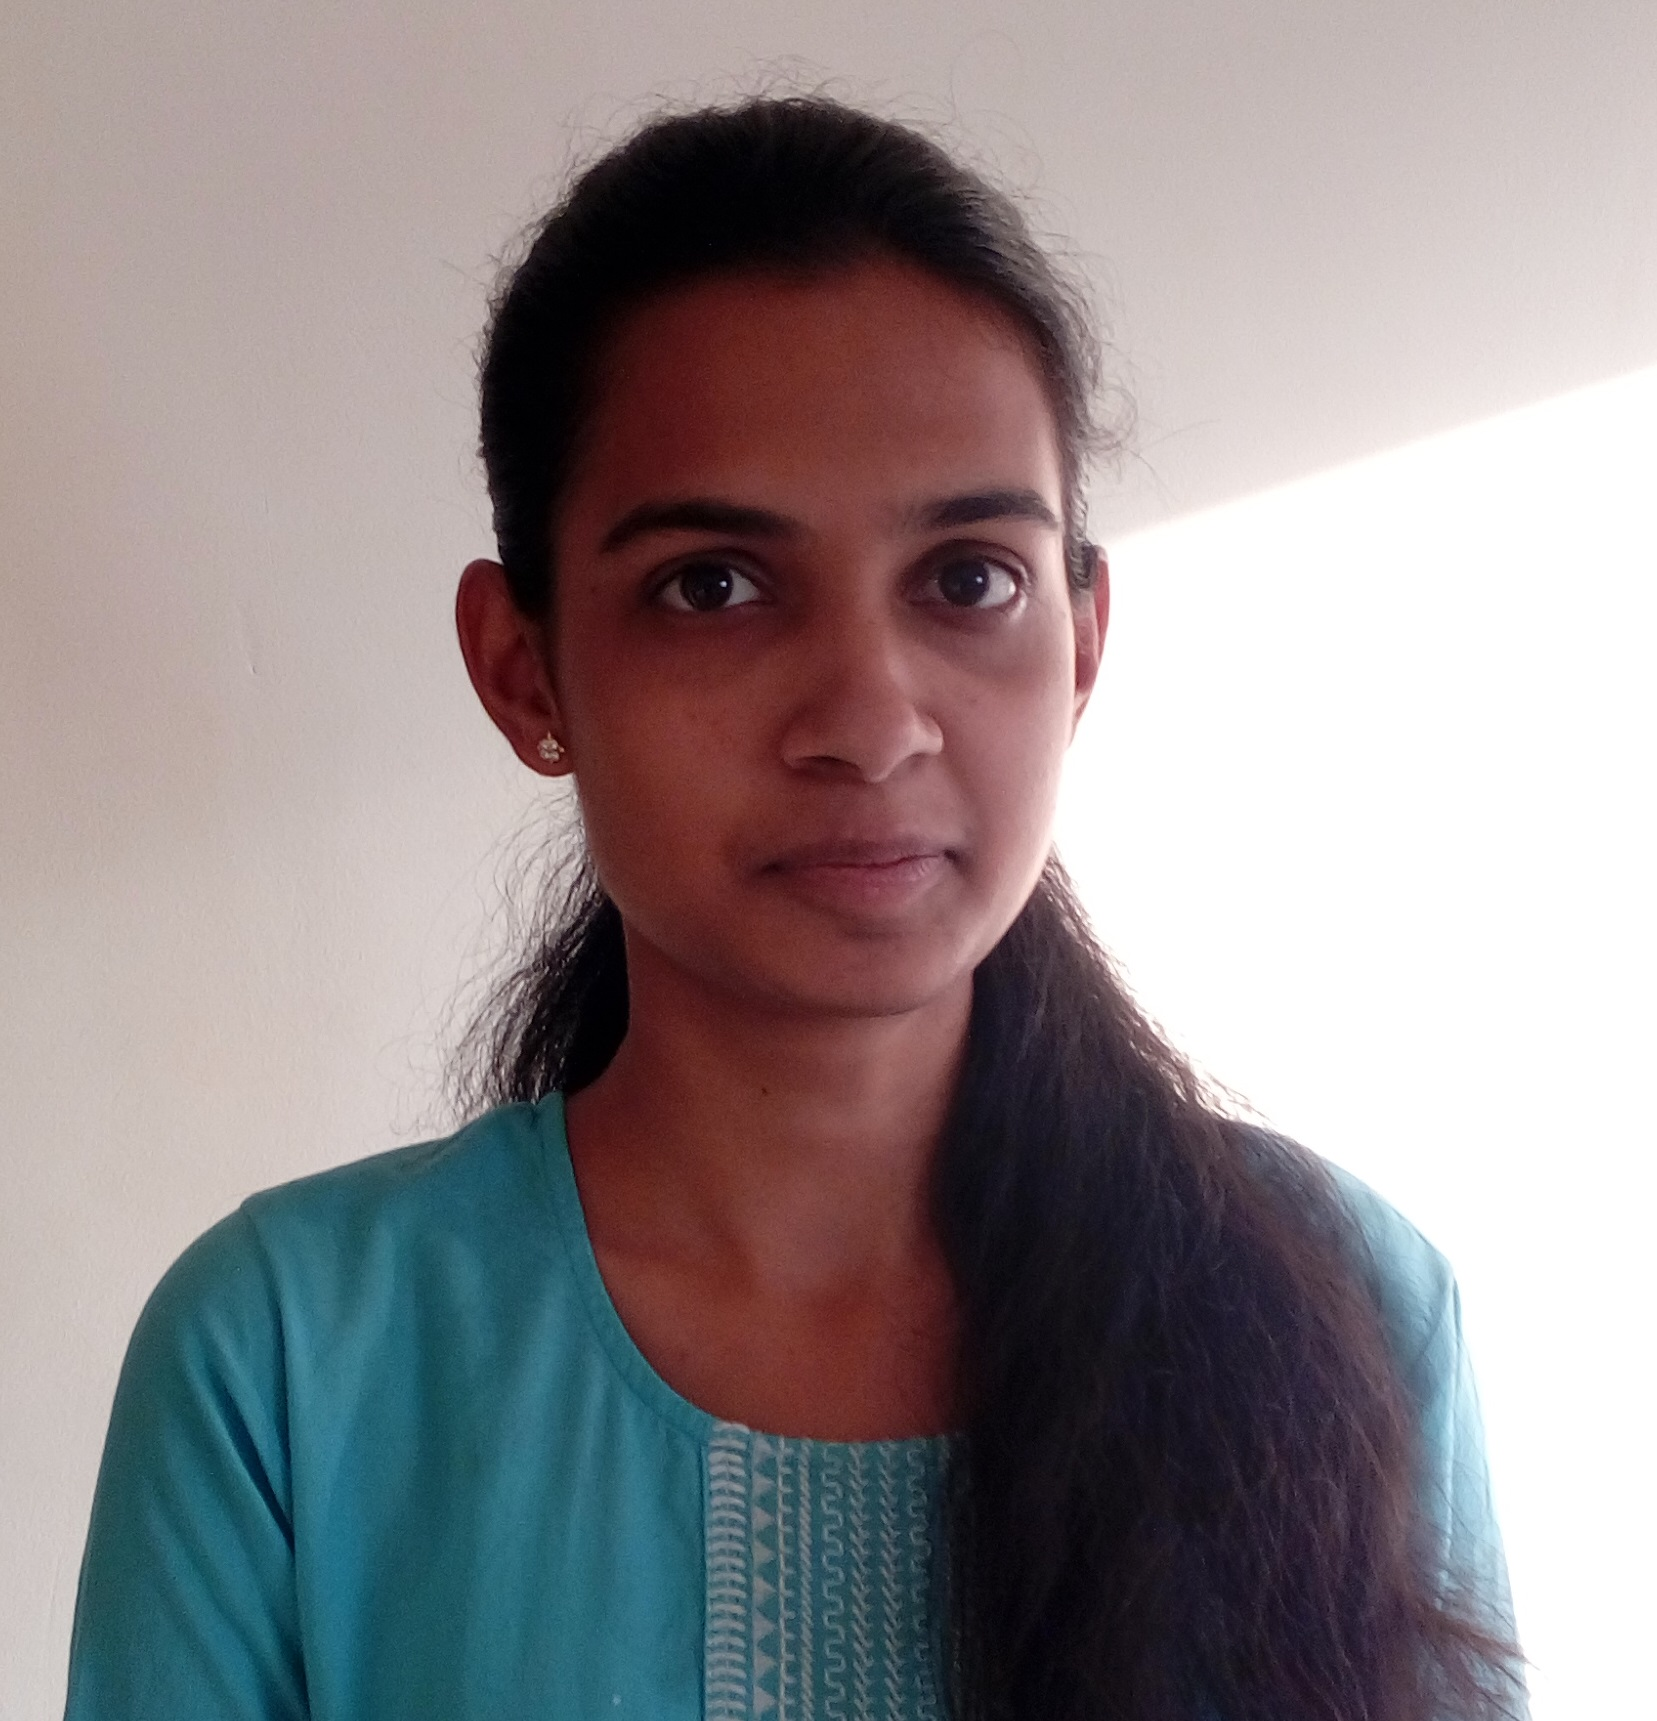
\includegraphics[scale=0.05]{profile}
\textbf{\LARGE Supriya Mane\\}\hfill
\\
\mbox{E-mail ID:\large supriya9597@gmail.com}\\
\mbox{Contact no:\large +91 7022900515}\\
\mbox{\large KLS GIT, Belagavi}\\
\paragraph{OBJECTIVE}
\line(1,0){400}\\
My goal is to pursue a career as an Electronics and Communication engineer in Embedded systems domain. Currently, I am looking for an internship where I can learn under professional guidance and also provide some inputs to the organization according to my skills.
\paragraph{EDUCATION}
	\line(1,0){400}
	\begin{itemize}
  		\item \textrm{X}(Secondary)\\
  			Year of Completion: 2013\\
			GOA BOARD OF SECONDARY AND HIGHER SECONDARY EDUCATION(St.Joseph's Institue)\\
			Percent: 91.8\verb"%"
  		\item \textrm{XII}(Higher Secondary)
  			Year of Completion: 2015\\
			GOA BOARD OF SECONDARY AND HIGHER SECONDARY EDUCATION(Mushtifund Higher Secondary School)\\
			Percent: 81.8\verb"%"
  		\item Bachelor of Engineering(B.E), Electronics and Communications(2015-2019)\\
  			  KLS Gogte Institute Of Technology\\
			  CGPA : 8.52/10(5th sem)
	\end{itemize}
\paragraph{PROJECTS}
	\line(1,0){420}
	\begin{itemize}
		\item \verb"[Current]Encryption techniques for IoT"
		\begin{itemize}
			\item Study of lightweight cryptography algorithms for IoT
			\item Implementing for TI Cc2650 or Cc2640R2F boards
			\item Comparing their performance with standard AES
		\end{itemize}
		\item Collector Bot-A bot that collects Fresh fruits avoiding damaged fruits and drop in Truck. It involved following components:
		\begin{itemize}
			\item A completely designed bot for moving and picking and dropping fruits
			\item Truck(Spark V)
			\item Use of ArUco Markers for simulation in Virtual Robot Experimentation Platform
			\item Python+VREP at Supervisor station to control Collector bot using Xbee\\
		\end{itemize}
	\end{itemize}

\end{document}